\documentclass[a4paper]{article}
\usepackage[utf8]{inputenc}
\usepackage[russian,english]{babel}
\usepackage[T2A]{fontenc}
\usepackage[left=10mm, top=20mm, right=18mm, bottom=15mm, footskip=10mm]{geometry}
\usepackage{indentfirst}
\usepackage{amsmath,amssymb}
\usepackage[italicdiff]{physics}
\usepackage{graphicx}
\graphicspath{{images/}}
\DeclareGraphicsExtensions{.pdf,.png,.jpg}
\usepackage{wrapfig}
\usepackage{pgfplots}

\usepackage{caption}
\captionsetup[figure]{name=Рисунок}
\captionsetup[table]{name=Таблица}


\title{\underline{Лабораторная работа 2.1.4}}
\author{Старостин Александр, Б01-401}
\date {19 Марта, 2025 год}


\begin{document}

\maketitle
\newpage

\textbf{Измерение теплоёкости твёрдого тела}

\section{Аннотация}
    \par \textbf{Цель работы:} 1. прямое измерение кривых нагревания $T_{heat}(t)$ и охлаждения $T_{cool}(T)$ пустого калориметра и системы «калориметр + твердое тело»; 2. определение коэффициента теплоотдачи стенок калориметра; 3. определение теплоемкости пустого калориметра и удельной теплоемкости твердого тела. \\

    \par \textbf{В работе используются:} калориметр с нагревателем и термометром сопротивления; универсальный вольтметр В7-78/3 в режиме омметра ($\sigma_{T} = 0.05~K$), измеритель температуры - термопара K-типа совместно с универсальным вольтметром В7-78/2 ($\sigma_{T_\text {комн}} = 0.1~K$), источник питания GPS-72303, универсальные вольтметры В7-78/3 (в режиме амперметра) ($\sigma_I = 0.01~A$) и KEITHLEY (в режиме вольтметра) ($\sigma_U = 0.1 \text{ В}$) для измерения мощности нагревателя, компьютерная программа АКИП для сопряжения персонального компьютера и универсальных вольтметров В7-78/2 и В7-78/3 ($\sigma_t = 0.01 \text{ с}$).

\section{Теоретические сведения}

          В данной работе теплоемкость определяется по формуле
        \begin{equation}
            C = \frac{\Delta Q}{\Delta T},
            \label{eq:dQdT}
        \end{equation}
        где $\Delta Q$ -- количество тепла, подведенного к телу, и $\Delta T$ -- изменение температуры тела, произошедшее в результате подвода тепла.

        Температура внутри калориметра измеряется термометром сопротивления. В реальных условиях $\Delta Q \neq P \Delta t$, так как часть энергии уходит из калориметра благодаря теплопроводности его стенок. В результате количество тепла $\Delta Q = C \Delta T$, подведённое к системе "тело + калориметр" будет меньше на величину тепловых потерь:

        \begin{equation}
            C \Delta T = P \Delta t - \lambda(T - T_к) \Delta T
            \label{eq:C_Delta_T}
        \end{equation}
        где $\lambda$ - коэффициент теплоотдачи стенок калориметра, $T$ - температура тела и калориметра, $T_к$ - комнатная температура.

        Уравнение (\ref{eq:C_Delta_T}) является основной расчетной формулой работы. В дифференциальной форме для процессов нагревания и охлаждения ($P = 0$) соответственно оно имеет следующий вид:

        \begin{align}
            C dT &= P dt - \lambda \left[ T_{heat}(t) - T_к(t) \right] dt \label{eq:CdT} \\
            C dT &= - \lambda \left[ T_{cool}(t) - T_к(t) \right] dt \label{eq:CdT2}
        \end{align}
        где $P$ ‒ мощность нагревателя, $\lambda$ ‒ коэффициент теплоотдачи стенок калориметра, $t$ – время, измеряемое от момента включения нагревателя, $T_{heat}(t)$ ‒ температура тела в момент времени $t$ на кривой нагревания, $T_{cool}(t)$ ‒ температура тела в момент времени $t$ на кривой охлаждения, $T_к(t)$ ‒ температура окружающего калориметр воздуха (комнатная) в момент времени $t$, $dt$ ‒ время, в течение которого температура тела изменилась на $dT$

\section{Ход работы}

  \subsection{Проведение измерений}

    \subsubsection{Охлаждение калориметра}

        Вставляем в калориметр охлаждённый конус. Через 4 минуты после того, как температура в калориметре начинает медленно расти, вынимаем конус и ждём ещё 4 минуты. Калориметр охладился примерно на $5 ^\circ\text{C}$.

    \subsubsection{Определение зависимости сопротивления терморезистора от времени при нагревании пустого калориметра}

        Включаем нагреватель, после того, как температура в калориметре превысила комнатную на $9^\circ\text{C}$, отключаем цепь спирали нагревателя.

    \subsubsection{Определение зависимости сопротивления терморезистора от времени при охлаждении пустого калориметра}

        Продолжаем следить за изменением температуры калориметра. После того, как она уменьшилась на 2 градуса по сравнению с максимальной, приступаем к измерению теплоёмкости калориметра вместе с исследуемым телом.

    \subsubsection{Охлаждение калориметра}

        Снова охлаждаем калориметр до температуры на $5^\circ\text{C}$ ниже комнатной. Вставляем в калориметр исследуемый образец и повторяем заново пункты 2-3.

    \subsubsection{Исследуемые образцы}

        Измерения проводим для образцов из алюминия и титана. Массы исследуемых образцов:

        \begin{align*}
            m_\text{алюм} &= (286.9 \pm 0.5) \text{ г} & m_\text{сталь} &= (812.8 \pm 0.5) \text{ г}
        \end{align*}

    \subsubsection{Окончание измерений}

        Останавливаем запись в программе. Сохраняем файлы с данным.

\subsection{Обработка результатов измерений}

\subsubsection{Временные интервалы}

    Сопоставим процессы с временными отметками:

    \begin{table}[!ht]
        \centering
        \begin{tabular}{|l|c|c|}
            \hline
            Событие & Начало, с & Конец, с\\ \hline
            $T_{heat_1}(t)$ - нагрев пустого калориметра & 780 & 2040\\ \hline
            $T_{cool_1}(t)$ - охлаждение пустого калориметра & 2040 & 2640\\ \hline
            $T_{heat_2}(t)$ - нагрев алюминия & 3840 & 5160\\ \hline
            $T_{cool_2}(t)$ - охлаждение алюминия & 5160 & 6240\\ \hline
            $T_{heat_3}(t)$ - нагрев стали & 7020 & 8580\\ \hline
            $T_{cool_3}(t)$ - охлаждение стали & 8580 & 8940\\ \hline

        \end{tabular}
        \caption{Сопоставление кривых с отметками времени}
        \label{tab:timetable}
    \end{table}

    Во время работы комнатная температура менялась менее чем на $2~K$, значит мы можем использовать интегральный способ вычисления теплоёмкости

   \subsubsection{Теплоёмкость пустого калориметра}

        Построим график ($ln \frac{T_{cool} - T_\text{к}}{T - T_\text{к}}$, $t$), где $T_\text{к}$ - среднее значение комнатной температуры за время измерения; $T$ - температура калориметра в начале кривой. \\
        \begin{figure}[ht]
            \centering
            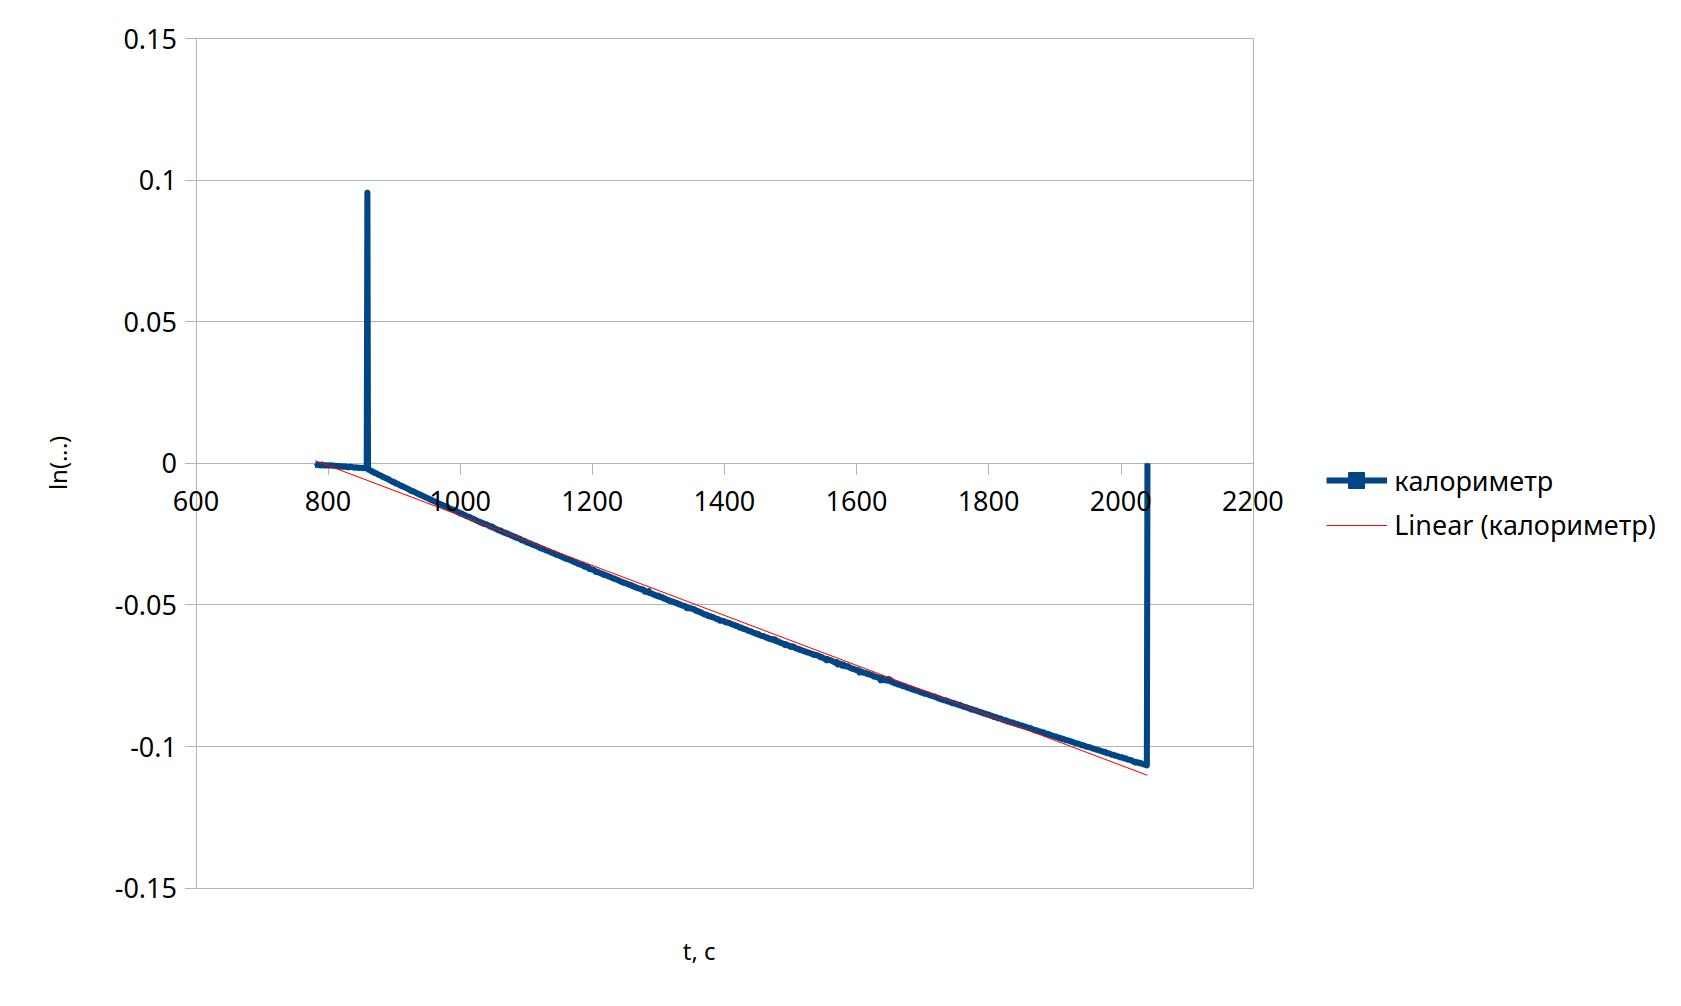
\includegraphics[width=0.6\textwidth]{калориметр.jpg}
            \caption{$T_{cool}(t)$ для пустого калориметра}
            \label{plot:T_cool_1}
        \end{figure}
        \\
        По МНК найдём коэффициент наклона $k$. Причём: \\

        $\frac{\lambda}{C} = -k$,

       \sigma_{\frac{\lambda}{C}}^\text{приб} = \sqrt{ \left( \frac{1}{t} \frac{\lambda}{C} \right)^2 \sigma_t^2 + \left( \frac{1}{t} \frac{1}{T_{cool} - T_\text{к}} \right)^2 \sigma_{T_{cool}}^2 + \left( \frac{1}{t} \frac{T_{cool} - T}{(T_{cool} - T_\text{к})(T - T_\text{к})} \right)^2 \sigma_{T_\text{к}}^2 + \left( \frac{1}{t} \frac{1}{T - T_\text{к}} \right)^2 \sigma_T^2}$,  \\

       Тогда: $\frac{\lambda}{C} = (88 \pm 25)*10^{-1} \text{ с}^{-1}$. \\

       Также  $\lambda = \frac{1}{k}$,

        $\sigma_{\lambda}^\text{приб} = \sqrt{\left( \frac{\lambda}{P} \right)^2 \sigma_P^2 + \left( \frac{P t e^{-\frac{\lambda}{C} t}}{T_{heat} - T_\text{к}} \right)^2 \sigma_{\frac{\lambda}{C}}^2 + \left( \frac{P \frac{\lambda}{C} e^{-\frac{\lambda}{C} t}}{T_{heat} - T_\text{к}} \right)^2 \sigma_t^2 + \left( \frac{\lambda}{T_{heat} - T_\text{к}} \right)^2 \left( \sigma_{T_{heat}}^2 + \sigma_{T_\text{к}}^2 \right)}$,

        $\sigma_C^\text{приб} = C \sqrt{\left( \frac{ \sigma_{\frac{\lambda}{P}}}{\frac{\lambda}{P}} \right)^2 + \left( \frac{\sigma_{\lambda}}{\lambda} \right)^2}$. \\

        Итого результат с полной погрешностью:

        $\lambda = (0.11 \pm 0.02)~\frac{\text{Дж}}{\text{К*с}}$,

        $C_\text{калориметр} = \lambda / \frac{\lambda}{C} = (0.79 \pm 0.07)~\frac{\text{кДж}}{\text{К}}$.  \\

\subsubsection{Теплоёмкость алюминия}

    Аналогично предыдущему пункту определяем теплоёмкость алюминиевого образца вместе с калориметром, затем вычитаем теплоёмкость калориметра.

    \begin{figure}[ht]
        \centering
        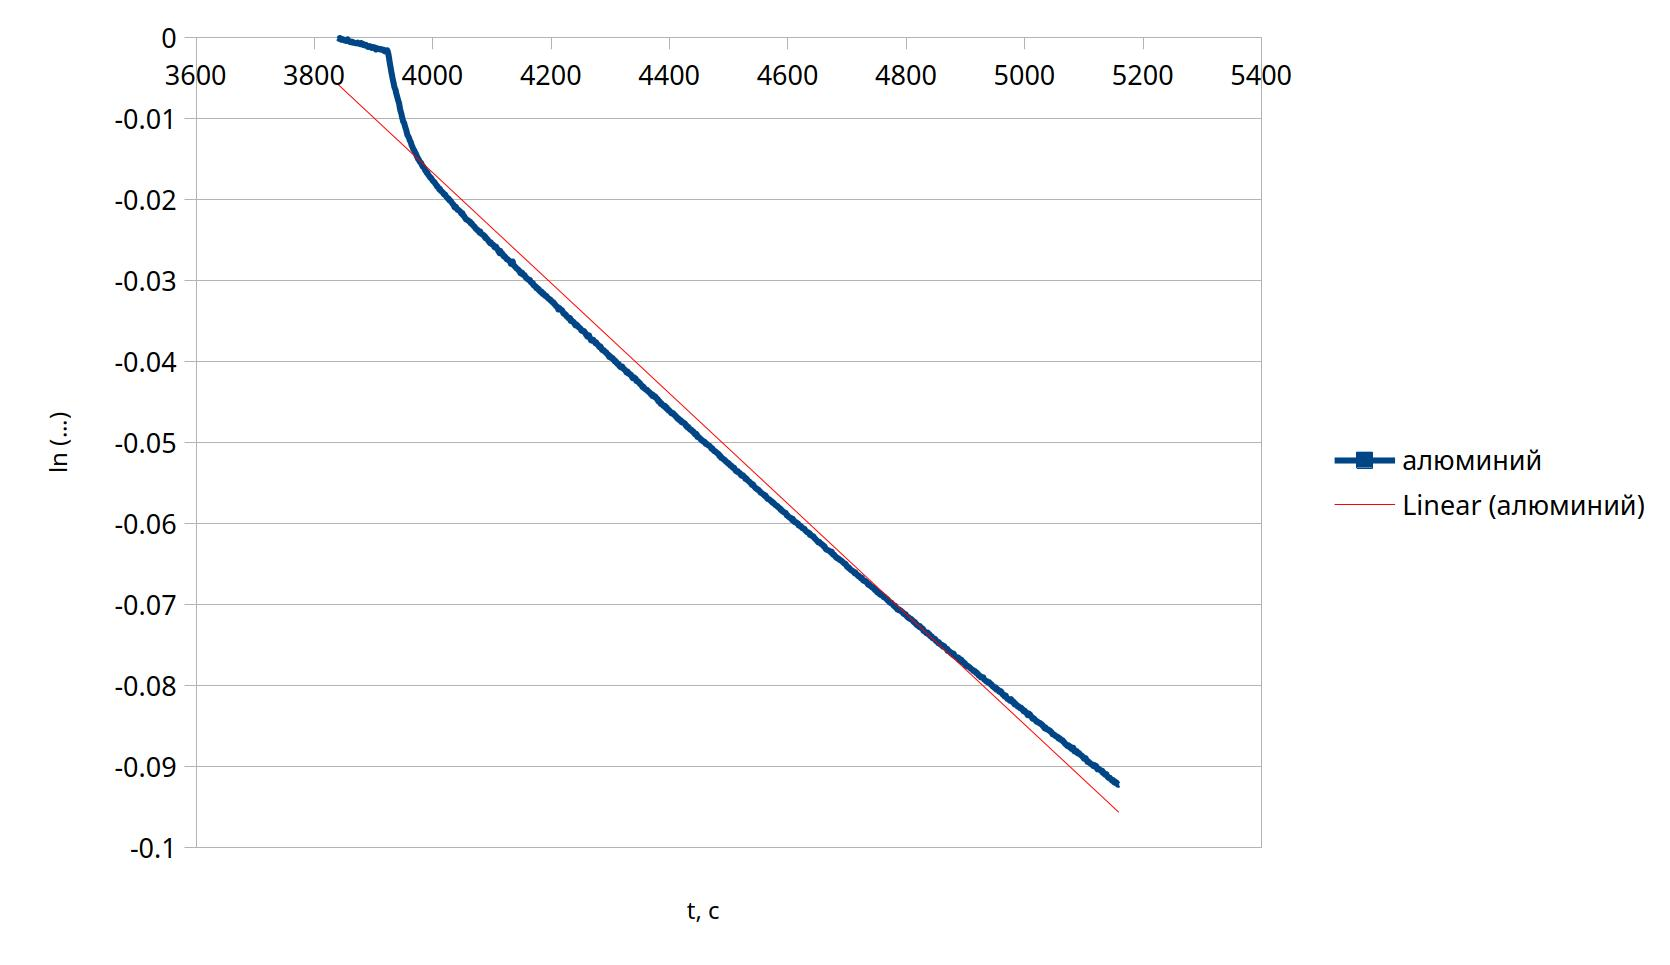
\includegraphics[width=0.6\textwidth]{алюминий.jpg}
        \caption{$T_{cool}(t)$ для калориметра с алюминиевым образцом}
        \label{plot:T_cool_2}
    \end{figure}

    Получаем: \\

    $\frac{\lambda}{C} = (68 \pm 20)*10^{-1} \text{ с}^{-1}$

    $\lambda = (0.15 \pm 0.03)~\frac{\text{Дж}}{\text{К*с}}$\\

    Тогда:

     $C = \lambda / \frac{\lambda}{C} = (1.0 \pm 0.2)~\frac{\text{кДж}}{\text{К}}$  \\

     И:

    $C_\text{алюм} = C - C_\text{калориметр} = (0.2 \pm 0.1)~\frac{\text{кДж}}{\text{К}}$

    $c_\text{алюм} = \frac{C_\text{алюм}}{m_{\text{алюм}}} = (0.8 \pm 0.6)~\frac{\text{кДж}}{\text{кг*К}}$


\subsubsection{Теплоёмкость стали}

    Аналогично найдём все нужные значения для стали.

    \newpage

    \begin{figure}[ht]
        \centering
        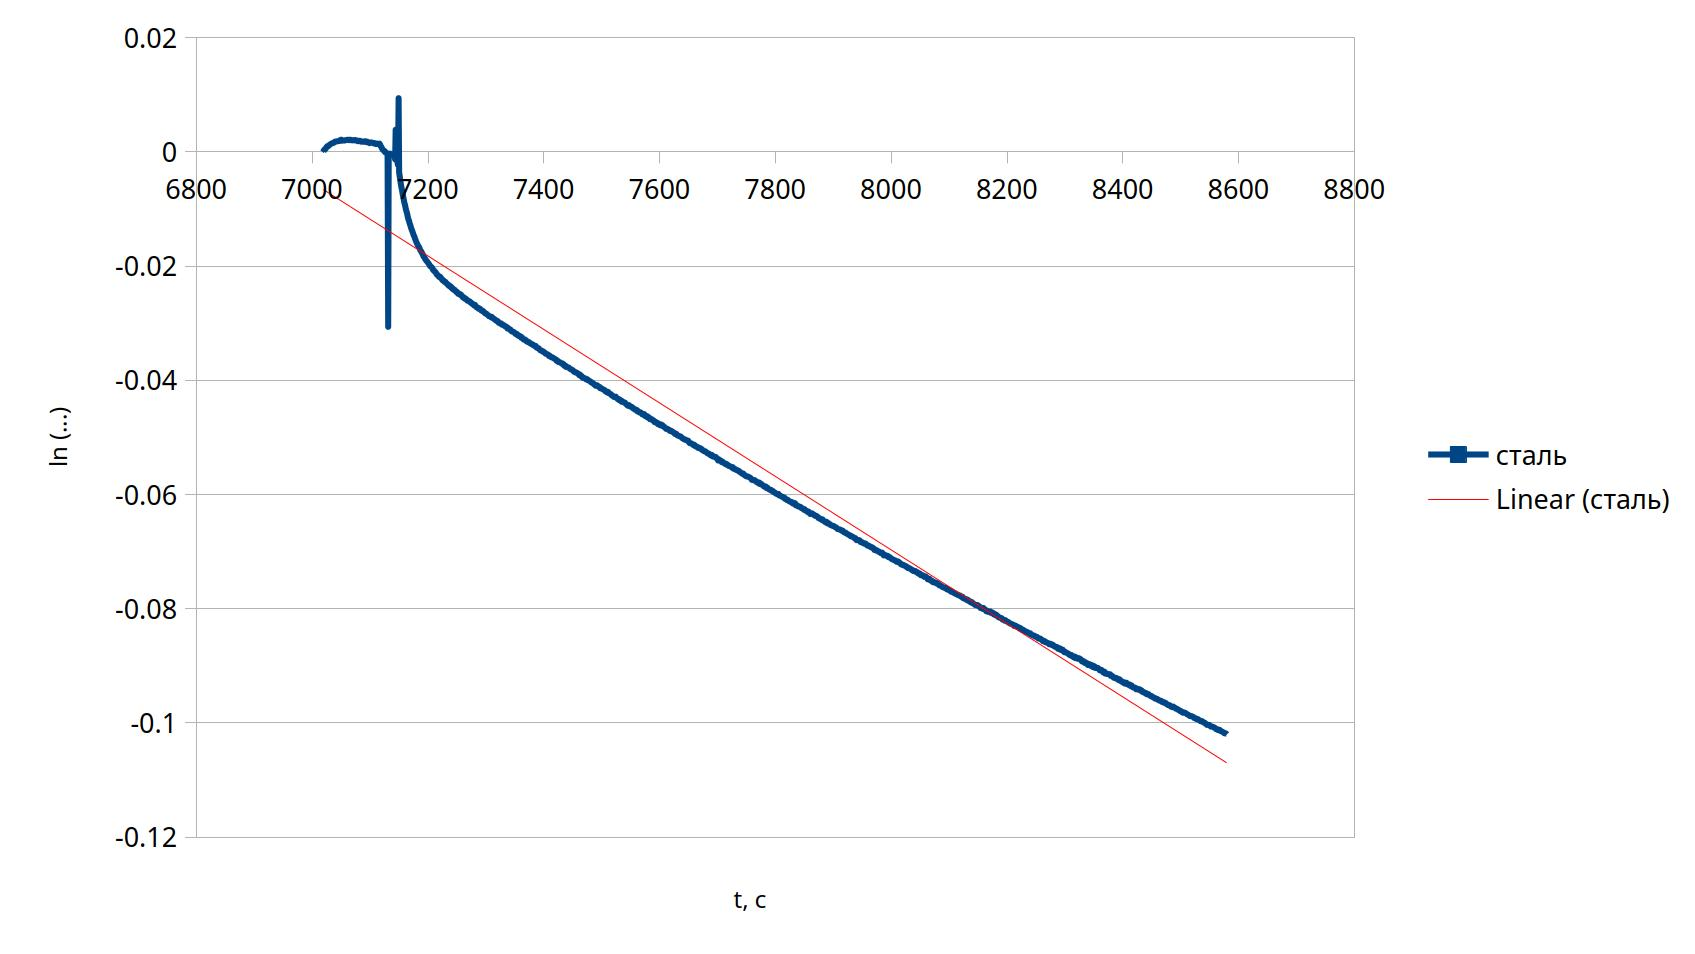
\includegraphics[width=0.6\textwidth]{сталь.jpg}
        \caption{$T_{cool}(t)$ для калориметра с титановым образцом}
        \label{plot:T_cool_3}
    \end{figure}

    Получаем:

    $\frac{\lambda}{C} = (64 \pm 16)*10^{-5}~\text{ с}^{-1}$,

    $\lambda = (0.16 \pm 0.04)~\frac{\text{Дж}}{\text{К*с}}$. \\

    Тогда:

    $C = \lambda / \frac{\lambda}{C} = (0.103\pm 0.245)~\frac{\text{кДж}}{\text{К}}$. \\

    И:

    $C_\text{сталь} = C - C_\text{калориметр} = (0.23 \pm 0.11)~\frac{\text{кДж}}{\text{К}}$,

    $c_\text{сталь} = \frac{C_\text{сталь}}{m_\text{сталь}} = (0.3 \pm 0.24)~\frac{\text{кДж}}{\text{кг*К}}$. \\

\section{Вывод}

Мы измерили удельные теплоёмкости алюминия и стали; они совпадают с табличными значениями. \\

Табличные значения удельных теплоёмкостей для алюминия и стали:

$c_\text{алюм} = 0.902~\frac{\text{кДж}}{\text{кг*К}}$,

$c_\text{сталь} = 0.462~\frac{\text{кДж}}{\text{кг*К}}$. \\

Результаты совпадают с табличными значениями. \\

Большая погрешность всех результатов объясняется тем, что мы производим вычитание теплоёмкости калориметра из суммарной теплоёмкости калориметра и образца. Из-за того, что теплоёмкость калориметра в несколько раз больше, и получаются погрешности порядка самих величин.

\end{document}

